%======================================================================
\NEWSEC
%======================================================================

\subsection{\ssScaling}

% \begin{frame}[fragile,label=ss-scaling] 
% \secframetitle{\ssScaling}
% \begin{center}
% \begin{minipage}{4.50in}
% 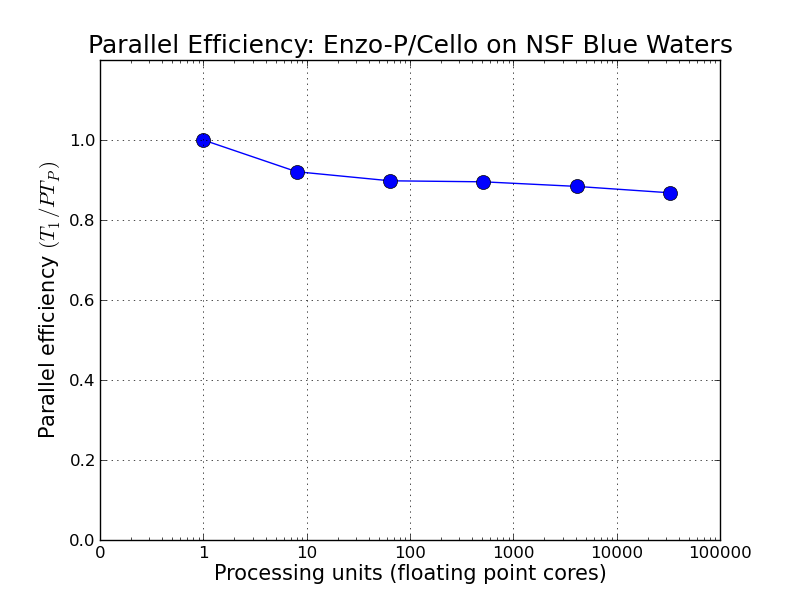
\includegraphics[width=2.25in]{Images/Scaling/scale-eff.png} \ 
% 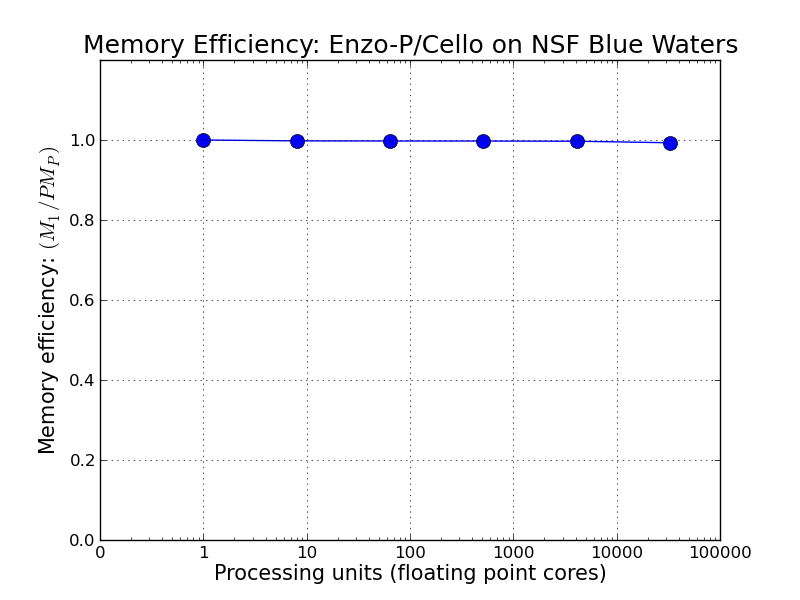
\includegraphics[width=2.25in]{Images/Scaling/scale-mem.png}
% \end{minipage} \\
% \begin{minipage}{4.0in}
% \footnotesize
% \pause
% \begin{minipage}[t]{1.20in}
% \blockblue
% \begin{block}<+->{Problem}
% %\begin{itemize}
% Sedov blast array \\
% $L=3$; $32K$ cores \\
% $32^3$ cells / block \\
% $329$ blocks /core
% %\end{itemize}
% \end{block}
% \end{minipage} \
% \begin{minipage}[t]{1.20in}
% \blockgreen
% \begin{block}<+->{Parallel Efficiency}
% %\begin{itemize}
% \begin{tabbing}
% xxxxxxxxxx\=\kill
% Time \> $0.868$ \\
% Memory \> $0.993$
% \end{tabbing}
% %\end{itemize}
% \end{block}
% \end{minipage} \
% \begin{minipage}[t]{1.20in}
% \blockred
% \begin{block}<+->{Caveats}
% %\begin{itemize}
% load balanced \\
% few refinement steps \\
% startup ignored
% %\end{itemize}
% \end{block}
% \end{minipage}
% \end{minipage}
% \end{center}
% \end{frame}

%----------------------------------------------------------------------

\begin{frame}[fragile]
 \secframetitle{\ssScaling}
  \framesubtitle{Hydro and tracer particles: ``Alphabet Soup'' problem}
%   \animategraphics[width=3.5in]{12}{de-2-}{0}{166} 
  \textbf{We tested basic \enzop\ hydrodynamics and particles scalability}
  \begin{minipage}{1.5in}
  \vspace{0.2in}
    \includegraphics<1>[width=1.5in]{Images/Scaling/de-2-3.png} \\
\ \\
    \includegraphics<1>[width=1.5in]{Images/Scaling/age-2-16.png}
  \end{minipage} \
  \begin{minipage}{2.80in}
    \vspace{0.1in}
    \begin{itemize}
    \item variation of ``array of Sedov Blast'' test
    \item letters instead of spheres
      \begin{itemize}
      \item inhibits lockstep coarsen/refine
      \end{itemize}
    \item one ``letter'' per Blue Waters core
    \item tested with/without tracer particles
    \item $32^3$ or $24^3$ cells per block
    \item decent sized AMR problem for 2016
      \begin{itemize}
      \item $256K$ fp-cores
      \item $1.7T$ cells; $0.7T$ (cells + particles)
        \item $50M$ Blocks
      \end{itemize}
      \item \enzo\ would need $72GB$ per process!
    \end{itemize}
    \end{minipage}
\end{frame}

\begin{frame}[fragile]
%--------------------------------------------------  
%--------------------------------------------------  
 \secframetitle{\ssScaling}
  \framesubtitle{Hydro and tracer particles: ``Alphabet Soup'' problem}
%--------------------------------------------------  
\begin{center}
  \vspace{-0.1in}
  \begin{minipage}{4.50in}
    \begin{center}
      \begin{minipage}{2in}
    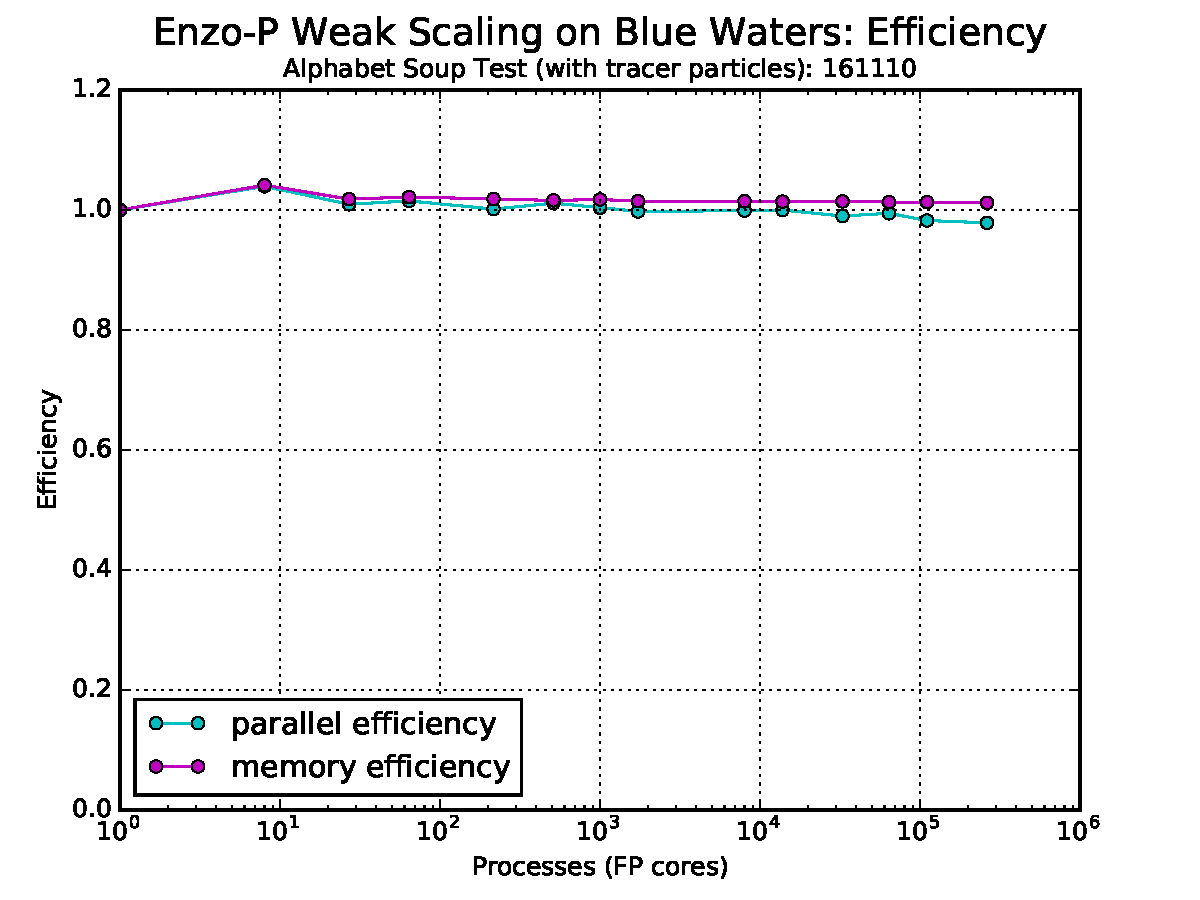
\includegraphics[width=2.0in]{Images/Scaling/scaling-efficiency-161110.pdf}
    \end{minipage} \ 
      \begin{minipage}{2in}
    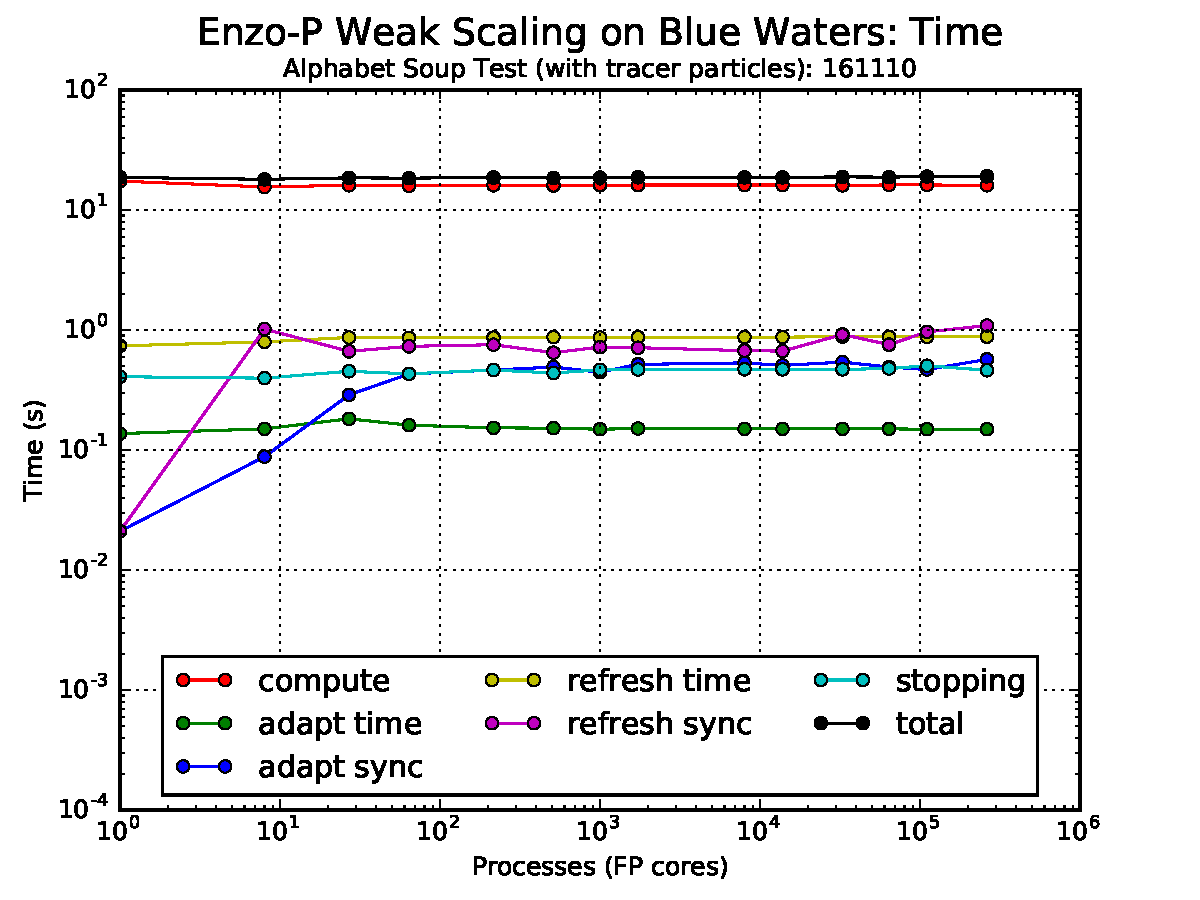
\includegraphics[width=2.0in]{Images/Scaling/scaling-time-161110.pdf}
    \end{minipage} \\
    \end{center}
  \end{minipage} \\
\end{center}
\end{frame}

%======================================================================

\begin{frame}[fragile]
%--------------------------------------------------  
 \secframetitle{\ssScaling}
\framesubtitle{Hydro, dark matterparticles, gravity: ``Cosmology (non-AMR)'' problem}
%--------------------------------------------------

\textbf{We tested scaling of more recent support for cosmology}

\begin{minipage}{1.5in}
  \vspace{0.2in}
  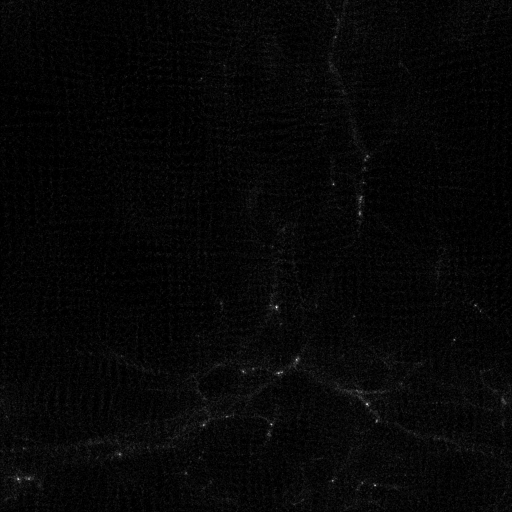
\includegraphics[width=1.5in]{Images/Cosmo/dark-20.png} \\
%\centerline{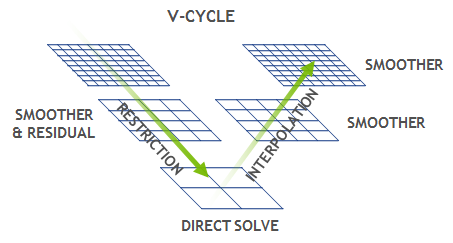
\includegraphics[width=1.5in]{hpgmg_v_cycle.png}}
\end{minipage} \
\begin{minipage}{2.75in}
  \vspace {0.2in}
  \begin{itemize}
  \item PPM hydrodynamics
  \item ``dark matter'' particles
  \item PM gravity method
  \item multigrid solver---non-AMR only
   \item tested up to $128K$ fp-cores
  \item have since implemented AMR solver
    \begin{itemize}
      \item Dan Reynolds ``HG'' algorithm
    \item preconditioned Krylov solver
    \item multigrid-based preconditioner
    \item effective up to $\approx 5$ levels
    \end{itemize}
  \end{itemize}
\end{minipage}
\end{frame}

%======================================================================

\begin{frame}[fragile]
  %--------------------------------------------------  
  \frametitle{\enzopcello\ NSF Blue Waters scaling}
  \framesubtitle{Hydro, particles, gravity: ``Cosmology (non-AMR)'' problem}
  %--------------------------------------------------  
  \begin{center}
    \vspace{-0.1in}
    \begin{minipage}{4.5in}
      \begin{center}
        \begin{minipage}{2.in}
          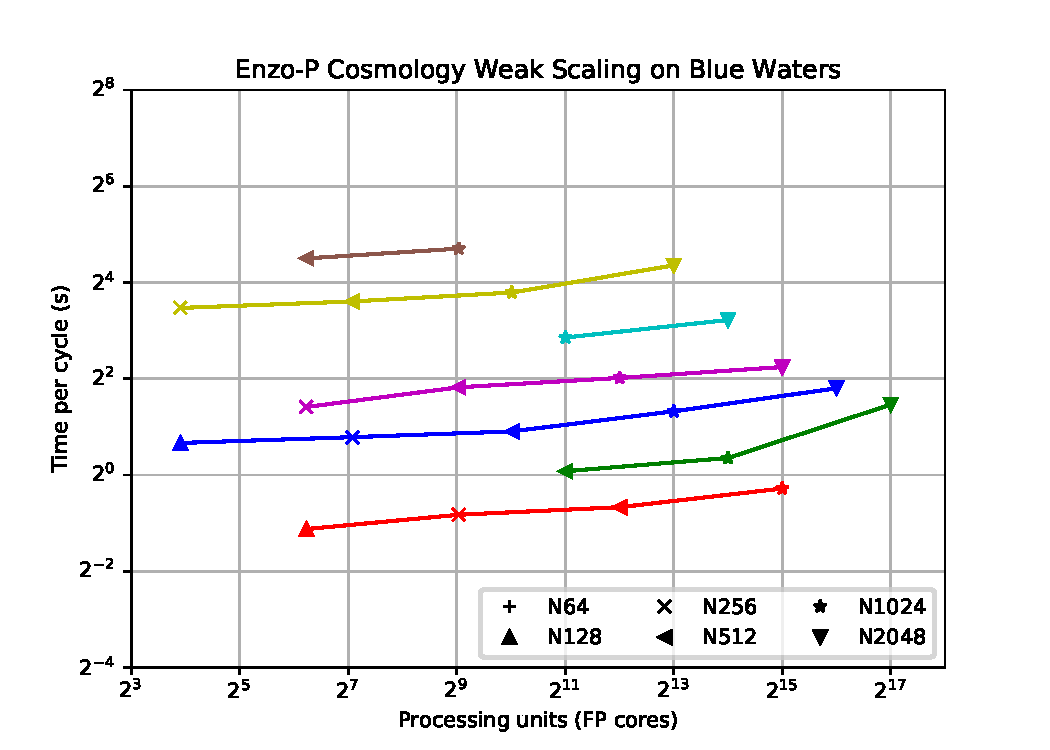
\includegraphics[width=2.2in]{Images/Scaling/smp-cosmo-weak.pdf}
        \end{minipage} \ 
        \begin{minipage}{2.2in}
          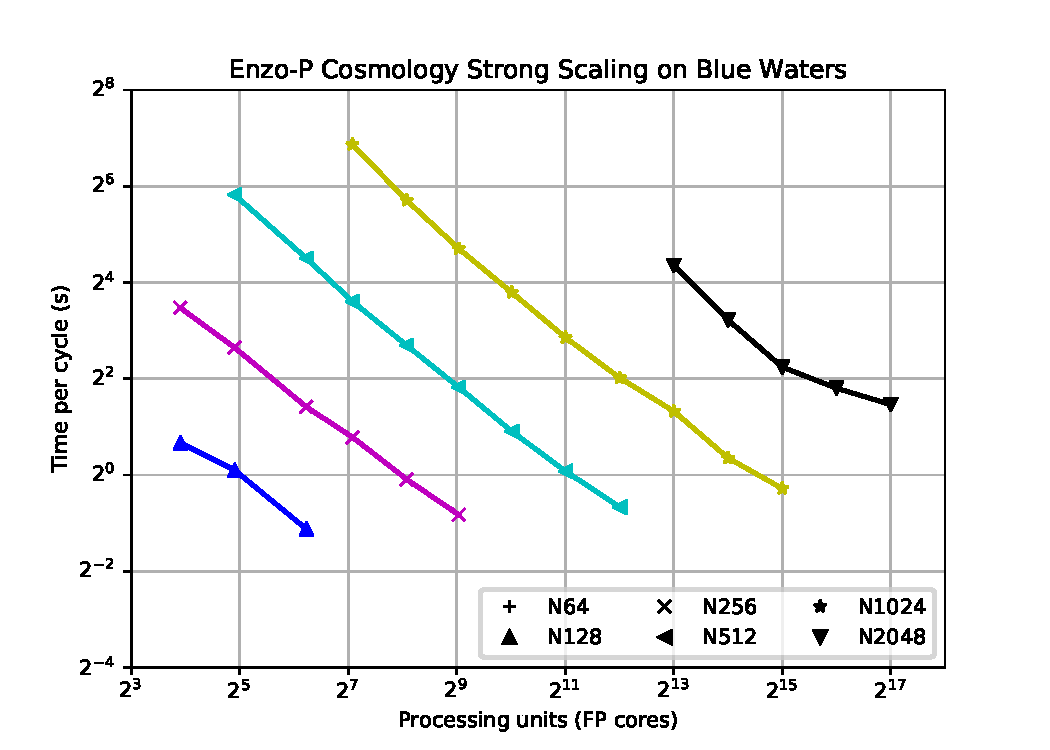
\includegraphics[width=2.2in]{Images/Scaling/smp-cosmo-strong.pdf}
        \end{minipage} \\
      \end{center}
    \end{minipage}
  \end{center}
\end{frame}

